\subsection{Graph Database} \label{subsec:graph_database}
% Checked - all edges are created with 'match' statement

% Intro
As we have created our base data models, our next objective~\ref{obj:graph_algorithm} is to create a graph database
that can be used to perform the PageRank algorithm as a graph algorithm.
With four huge datasets at our disposal, optimizing the generation of the database is crucial.
In this section, we describe the queries, called cypher queries, used to create and populate our graph database,
including information about creating indexes, constraints, relationships between nodes, and loading data into the database.\\


% PPI Network
\subsubsection*{basic PPI network} \label{subsubsec:basic_ppi_network}
To construct the \textbf{basic PPI network}, we need to create protein nodes and their interactions as edges.
To optimize query execution, we start with indexing the protein property $ID$.
Next we load the data (\cref{subsubsec:protein_nodes}~-~Protein nodes) as a list and then create the nodes in batches for efficient processing.
The graph database is populated with 104,235 protein nodes.

Since these nodes are used solely for connections between genes, no additional properties are required.
The cypher query for creating protein nodes is:
\begin{lstlisting}[language=Cypher, label={lst:protein_nodes}]
    CREATE (p:protein {id: 'Protein ID'})
\end{lstlisting}
\vspace{\baselineskip}

We then create interaction edges by loading the saved data (\cref{subsubsec:protein_protein_edges}~-~Protein-protein edges)
as a list of protein tuples and searching for both protein nodes by their ID in the graph database.
The edges are created in batches for efficient processing, resulting in 11,247,242 interactions between protein nodes.

The cypher query for creating protein-protein edges is:
\begin{lstlisting}[language=Cypher, label={lst:protein_edges}]
    MATCH (s:protein{id:'left Protein ID'})
    MATCH (s:protein{id:'right Protein ID'})
    CREATE (s)-[:interaction]->(t)
\end{lstlisting}

We now have a complete PPI network in place.\\

% MATCH p=()-[r:interaction]->() RETURN p LIMIT 5
\begin{figure}[h]
    \centering
    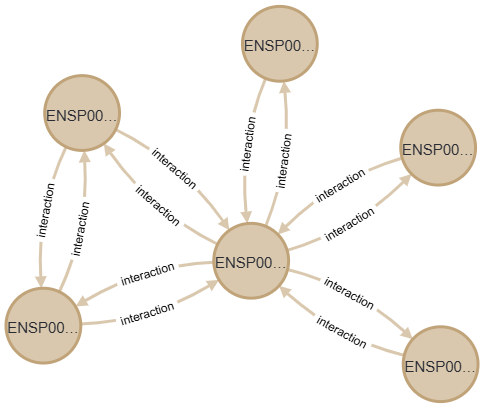
\includegraphics[width=0.35\textwidth]{figures/03_03_Basic_Network}
    \caption{Extract from the graph database setup showing example protein nodes and their interactions}
    \label{fig:03_03_Basic_Network}
\end{figure}
\vspace{\baselineskip}


%%%%%%%%%%%%%%%%%%%%%%%%%%%%%%%%%%%%%%%%%%%%%%%%%%%%%%%%%%%%%%%%%%%%%%%%%%%%%%%%%%%%%%%%%%%%%%%%%%%%%%%%%
% Extending the Network with Genes
\subsubsection*{extended PPI network} \label{subsubsec:extended_ppi_network}
To construct our \textbf{extended PPI network} we need to integrate genes into the created protein network.

First, we implement an index on the gene property $ID$ for faster querying.
We load the saved data (\cref{subsubsec:gene_nodes}~-~Gene nodes) as a list and create 17,626 gene nodes
in batches with their properties.

The cypher query employed for creating these gene nodes is:
\lstset{literate={Δ}{{\ensuremath{\Delta}}}1}
\begin{lstlisting}[language=Cypher, label={lst:gene_nodes}]
    CREATE (p:gene {
            id: 'Gene ID',
            gene_name: 'Gene Name',
            norm_healthy_tpm: 'norm healthy TPM',
            norm_cancerous_tpm: 'norm cancerous TPM',
            delta_tpm: 'Δ TPM',
            delta_type: 'Δ type',
            z_score: 'z score',
            delta_tpm_relevant: 'Δ TPM relevant'})
\end{lstlisting}

We characterize the genes in our network using these properties:
$gene\_name$, $norm\_healthy\_tpm$, $norm\_cancerous\_tpm$, $delta\_tpm$, $delta\_type$, $z\_score$, and $delta\_tpm\_relevant$.


Among these, the value of $delta\_tpm\_relevant$ stands out as a pivotal factor in our analysis.
Although other attributes may be less relevant to our current investigation, they retain potential value for future tasks.\\

To model relationships between genes and proteins,
we establish edges between these nodes by loading the gene-protein interaction data
(\cref{subsubsec:gene_protein_connections}~-~Gene-protein edges) as a list of tuples.
This involves matching gene and protein nodes based on their respective IDs,
and creating edges in batches to optimize processing efficiency.
The result is a comprehensive network of 101,731 connections between gene and protein nodes.

The cypher query for creating gene-protein connection edges is:
\begin{lstlisting}[language=Cypher, label={lst:gene_protein_edges}]
    MATCH (s:protein{id:'Protein ID'})
    MATCH (s:gene{id:'Gene ID'})
    CREATE (s)-[:connection]-(t)
\end{lstlisting}

\begin{figure}[h]
    \centering
    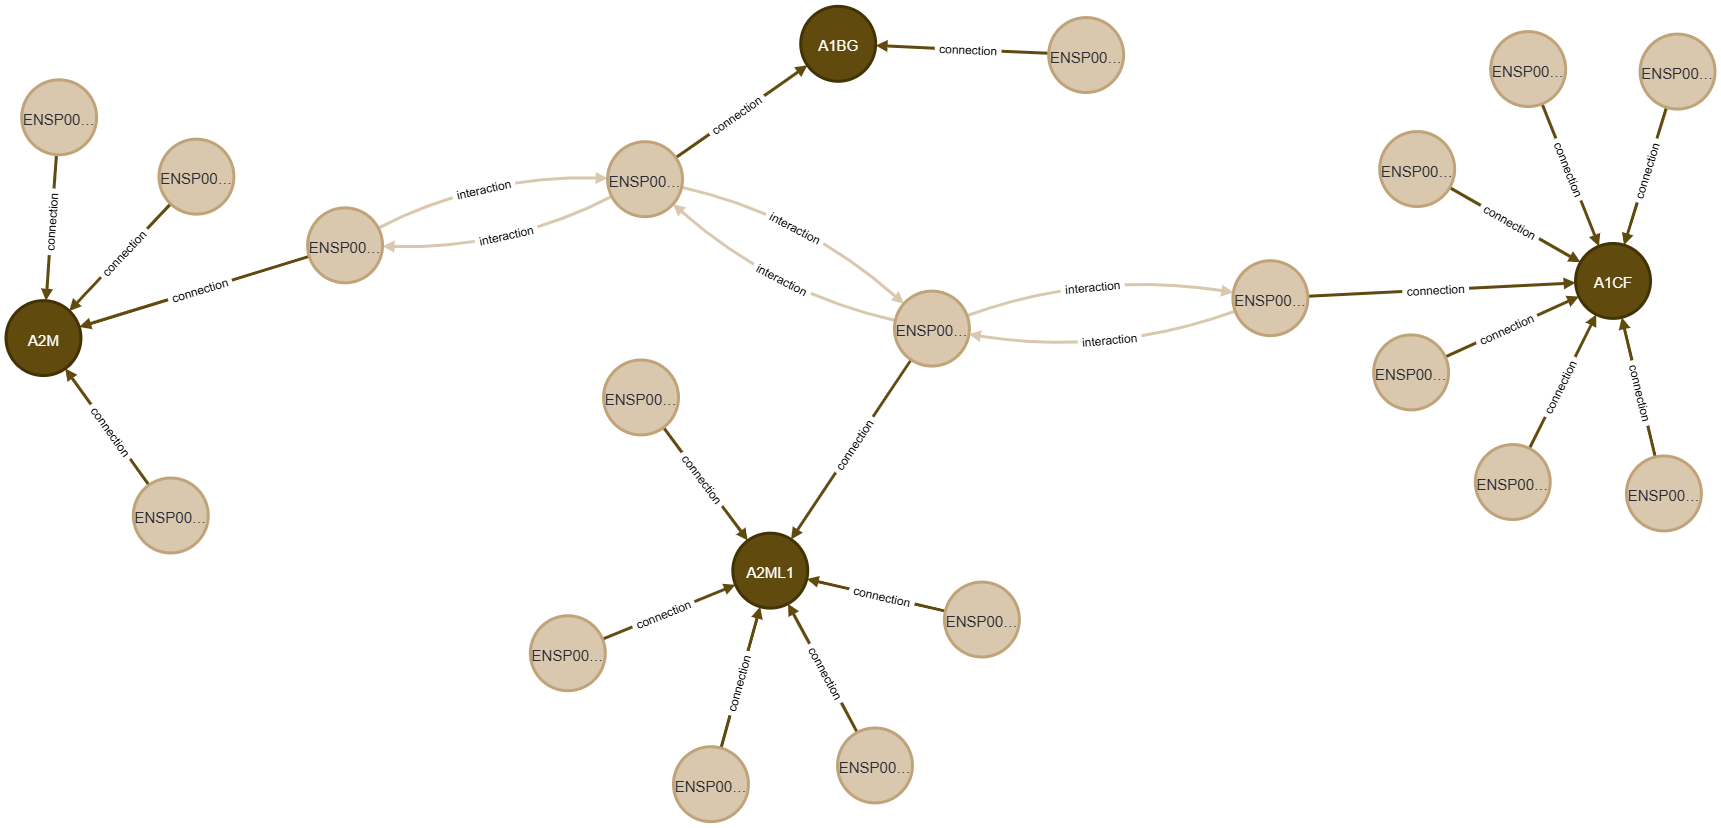
\includegraphics[width=1\textwidth]{figures/03_02_Network_2}
    \caption{Extract from the graph database setup showing example gene nodes and their connections to protein nodes}
    \label{fig:03_02_Network_2}
\end{figure}

Through the execution of these cypher queries,
we successfully populate our graph database with the required nodes and edges, enabling us to perform the PageRank algorithm.\\